\section{Results}
\label{sec:Results}

\subsection{Simulated Geometries}

The simulated count for the detector designs is shown in Figure ~\ref{fig:SimCountRate}\todo{Change to CPS, not interactions}, with the values enumerated in Table \ref{tab:MCNPXCountRatePerMg}.
Not that this value does not include the scaling necessary to achieve the gamma discrimination. 
It is immediately obvious that as the maximum total count rate occurs when the most \iso[6]{Li} is present in the detector, this occurs when 6 assemblies are spaced \si{\centi\meter} from each other.
However, this is also the least efficient use of the \iso[6]{Li}.
The most efficient use of the neutron absorber requires the flux to be thermalized in order to have a high probability of interaction.
Thus, it is expected that 1 film per assembly spaced \SI{4}{\centi\meter} apart would have the the largest count rate per absorber mass.
However, it was observed in Figure ~\ref{fig:SimCountRate} that one film per assembly with assemblies spaced \SI{3}{\centi\meter} apart had the highest count rate per \si{\milli\gram} \iso[6]{Li}.
In both cases only 3 assemblies fit into the RPM8 module.
It is then thought that the additional reflector material with the assemblies spaced \SI{3}{\centi\meter} apart caused more neutrons to cross the last film.
\begin{figure}
    \centering
    \begin{subfigure}[b]{0.45\textwidth}
        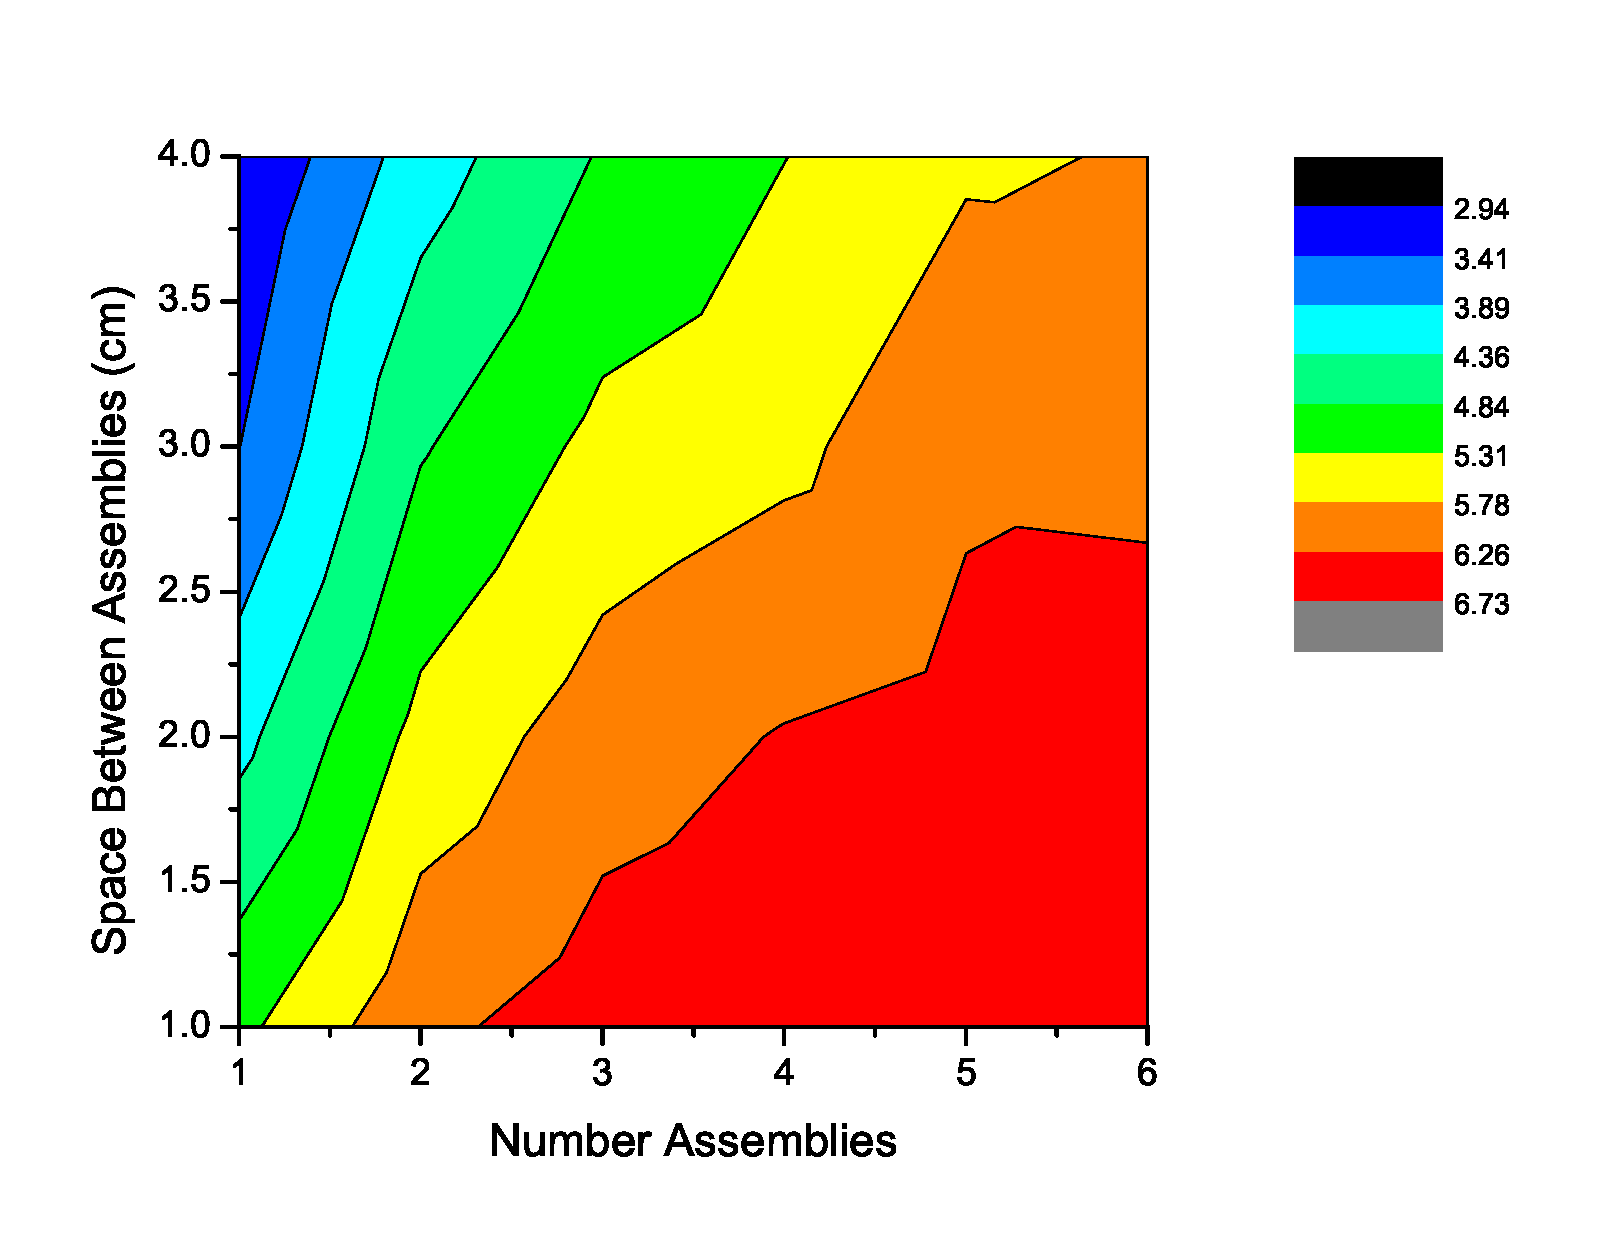
\includegraphics[width=\textwidth]{RPM8Opt_CR.eps}
        \caption{Count Rate per \si{\nano\gram\iso[252]{Cf}}}
    \end{subfigure}%
    ~
    \begin{subfigure}[b]{0.45\textwidth}
        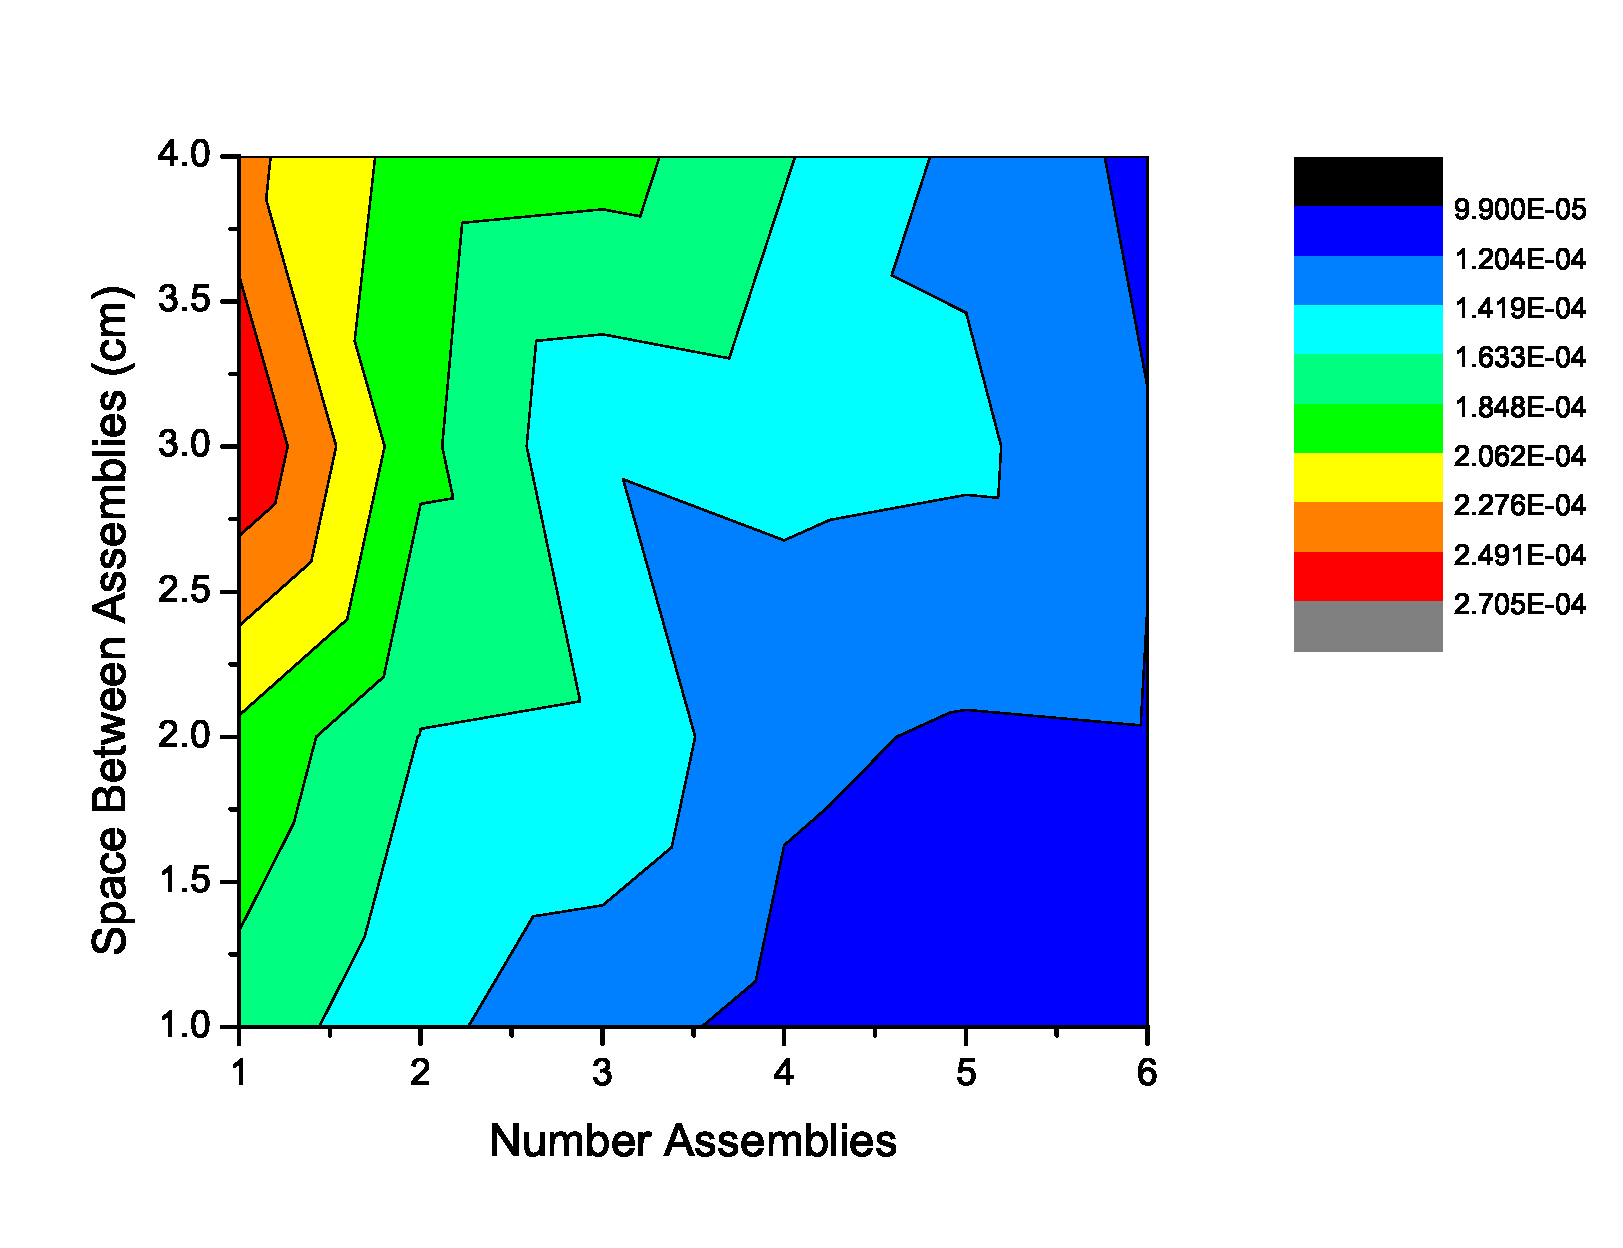
\includegraphics[width=\textwidth]{RPM8Opt_CRperLi.eps}
        \caption{Count Rate per nano gram \iso[252]{Cf} per \si{\milli\gram} \iso[6]{Li}}
    \end{subfigure}
    \caption{Count rate per dependence on number of assemblies and spacing of the simulated detectors. The amount of \iso[6]{Li} is not constant}
    \label{fig:SimCountRate}
\end{figure}
\begin{table}
  \caption{Count Rate per nano gram \iso[252]{Cf} per \si{\milli\gram} \iso[6]{Li} for the MCNPX simulated geometries}
	\label{tab:MCNPXCountRatePerMg}
  \centering
	\input{CountRatePerMg.dat}
\end{table}

\begin{figure}
	\centering
	\begin{subfigure}[b]{0.43\textwidth}
		\centering
		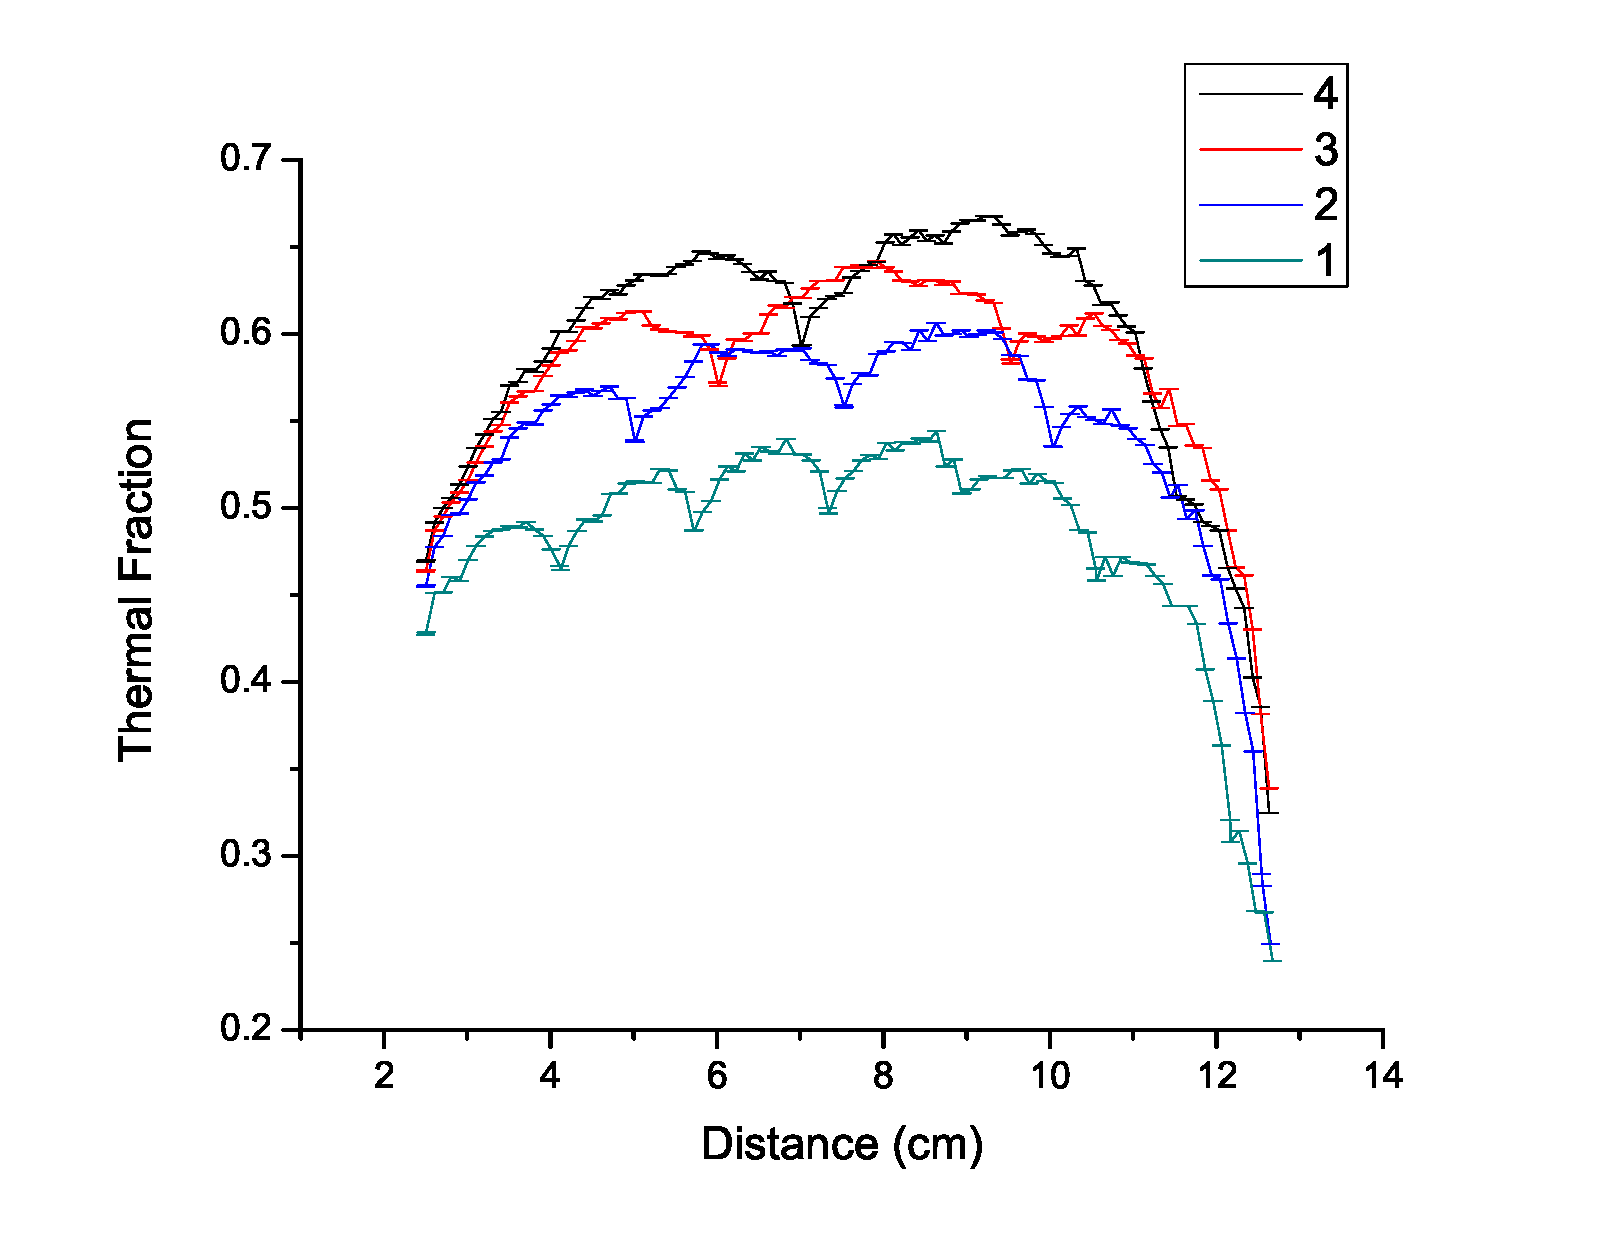
\includegraphics[width=\textwidth]{RPM8Opt_TF_1Assm.eps}
    \caption{1 Films per Assembly}
	\end{subfigure}%
	~
	\begin{subfigure}[b]{0.43\textwidth}
		\centering
		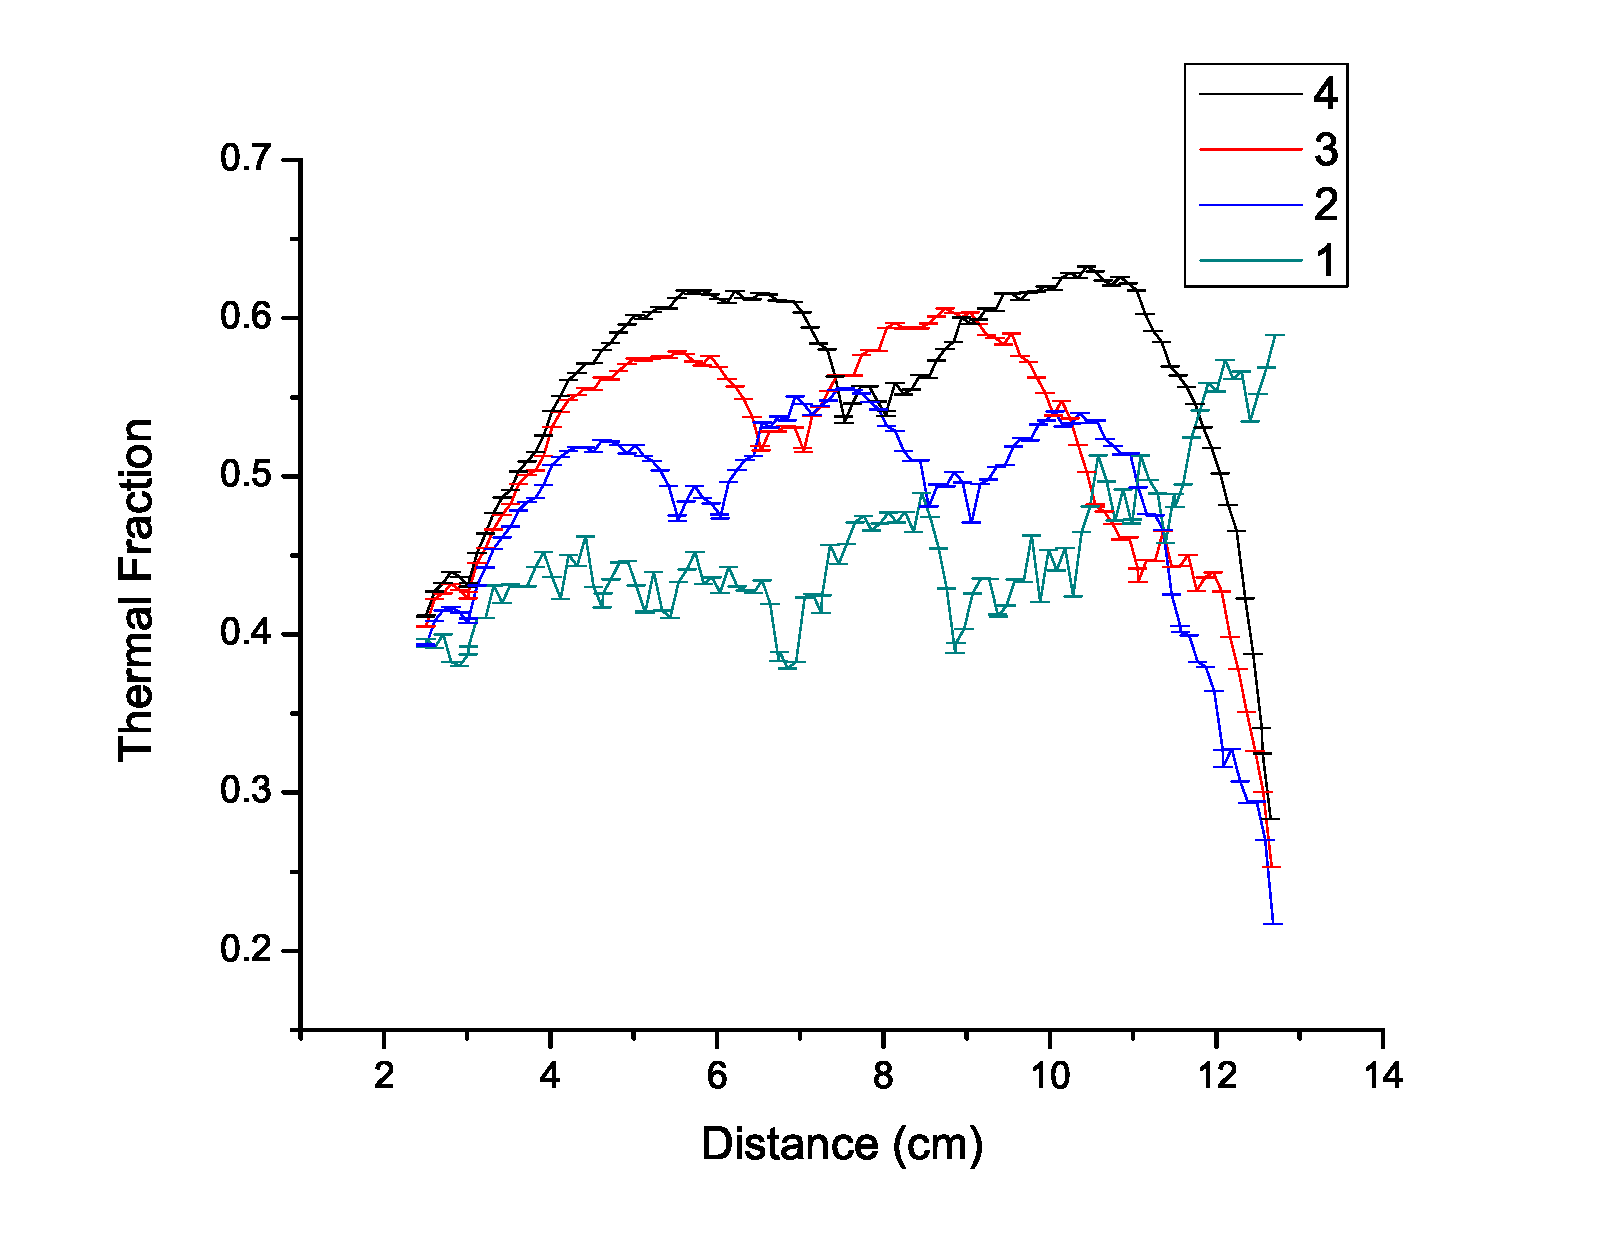
\includegraphics[width=\textwidth]{RPM8Opt_TF_2Assm.eps}
    \caption{2 Films per Assembly}
	\end{subfigure}	
	
  \begin{subfigure}[b]{0.43\textwidth}
		\centering
		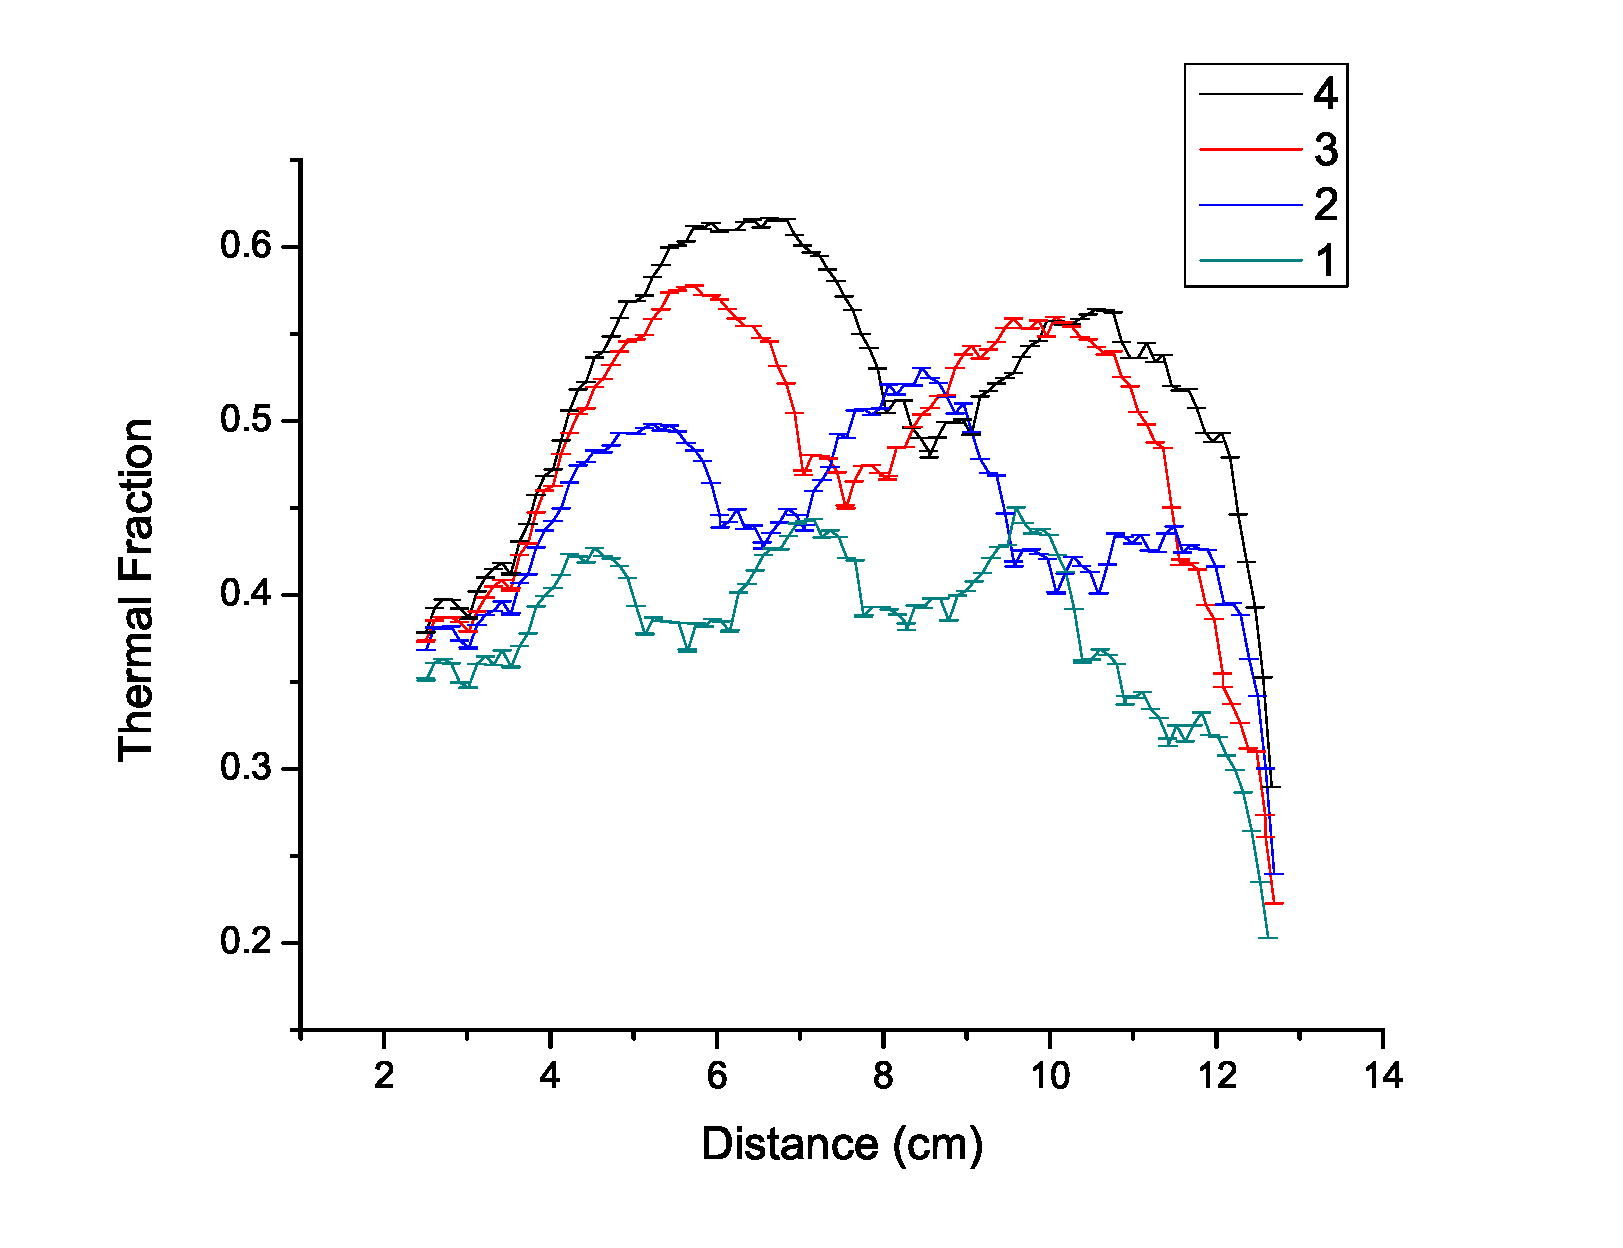
\includegraphics[width=\textwidth]{RPM8Opt_TF_3Assm.eps}
    \caption{3 Films per Assembly}
	\end{subfigure}%
	~
	\begin{subfigure}[b]{0.43\textwidth}
		\centering
		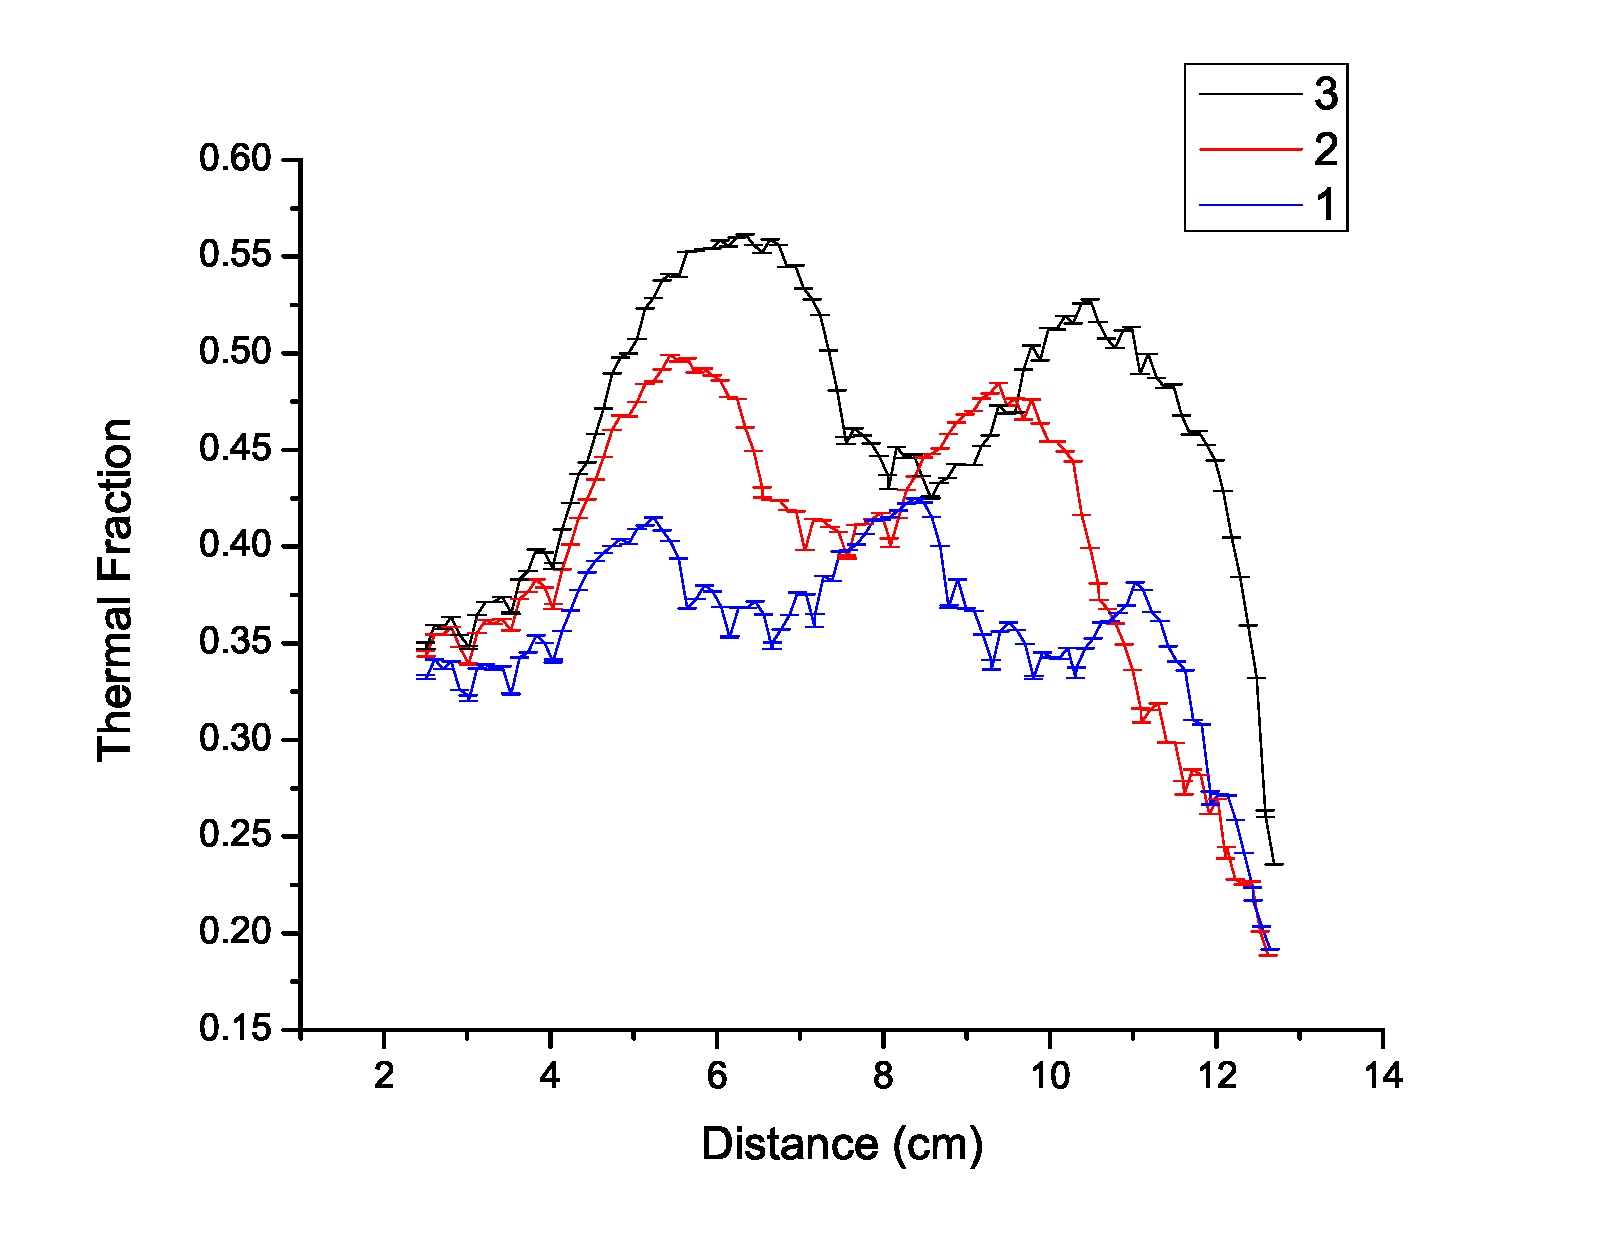
\includegraphics[width=\textwidth]{RPM8Opt_TF_4Assm.eps}
    \caption{4 Films per Assembly}
	\end{subfigure}	

	\begin{subfigure}[b]{0.43\textwidth}
		\centering
		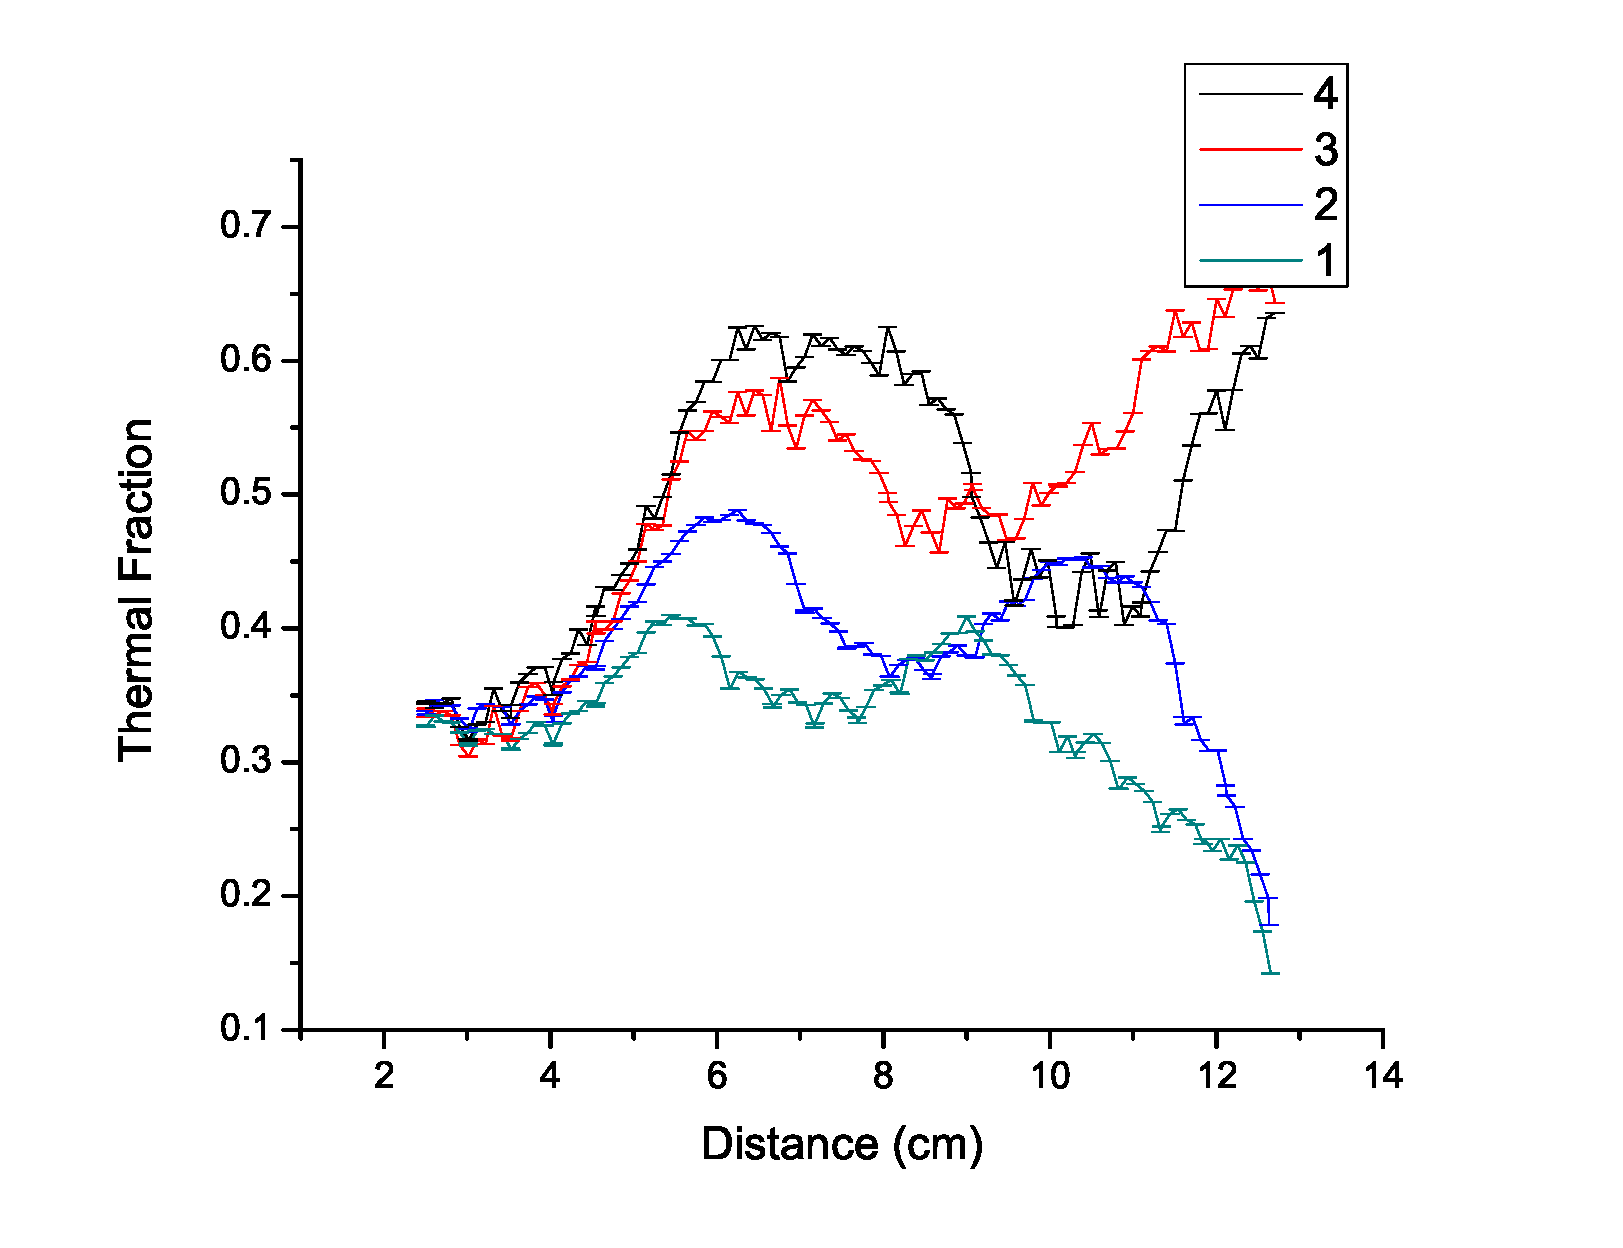
\includegraphics[width=\textwidth]{RPM8Opt_TF_5Assm.eps}
    \caption{5 Films per Assembly}
	\end{subfigure}%
	~
	\begin{subfigure}[b]{0.43\textwidth}
		\centering
		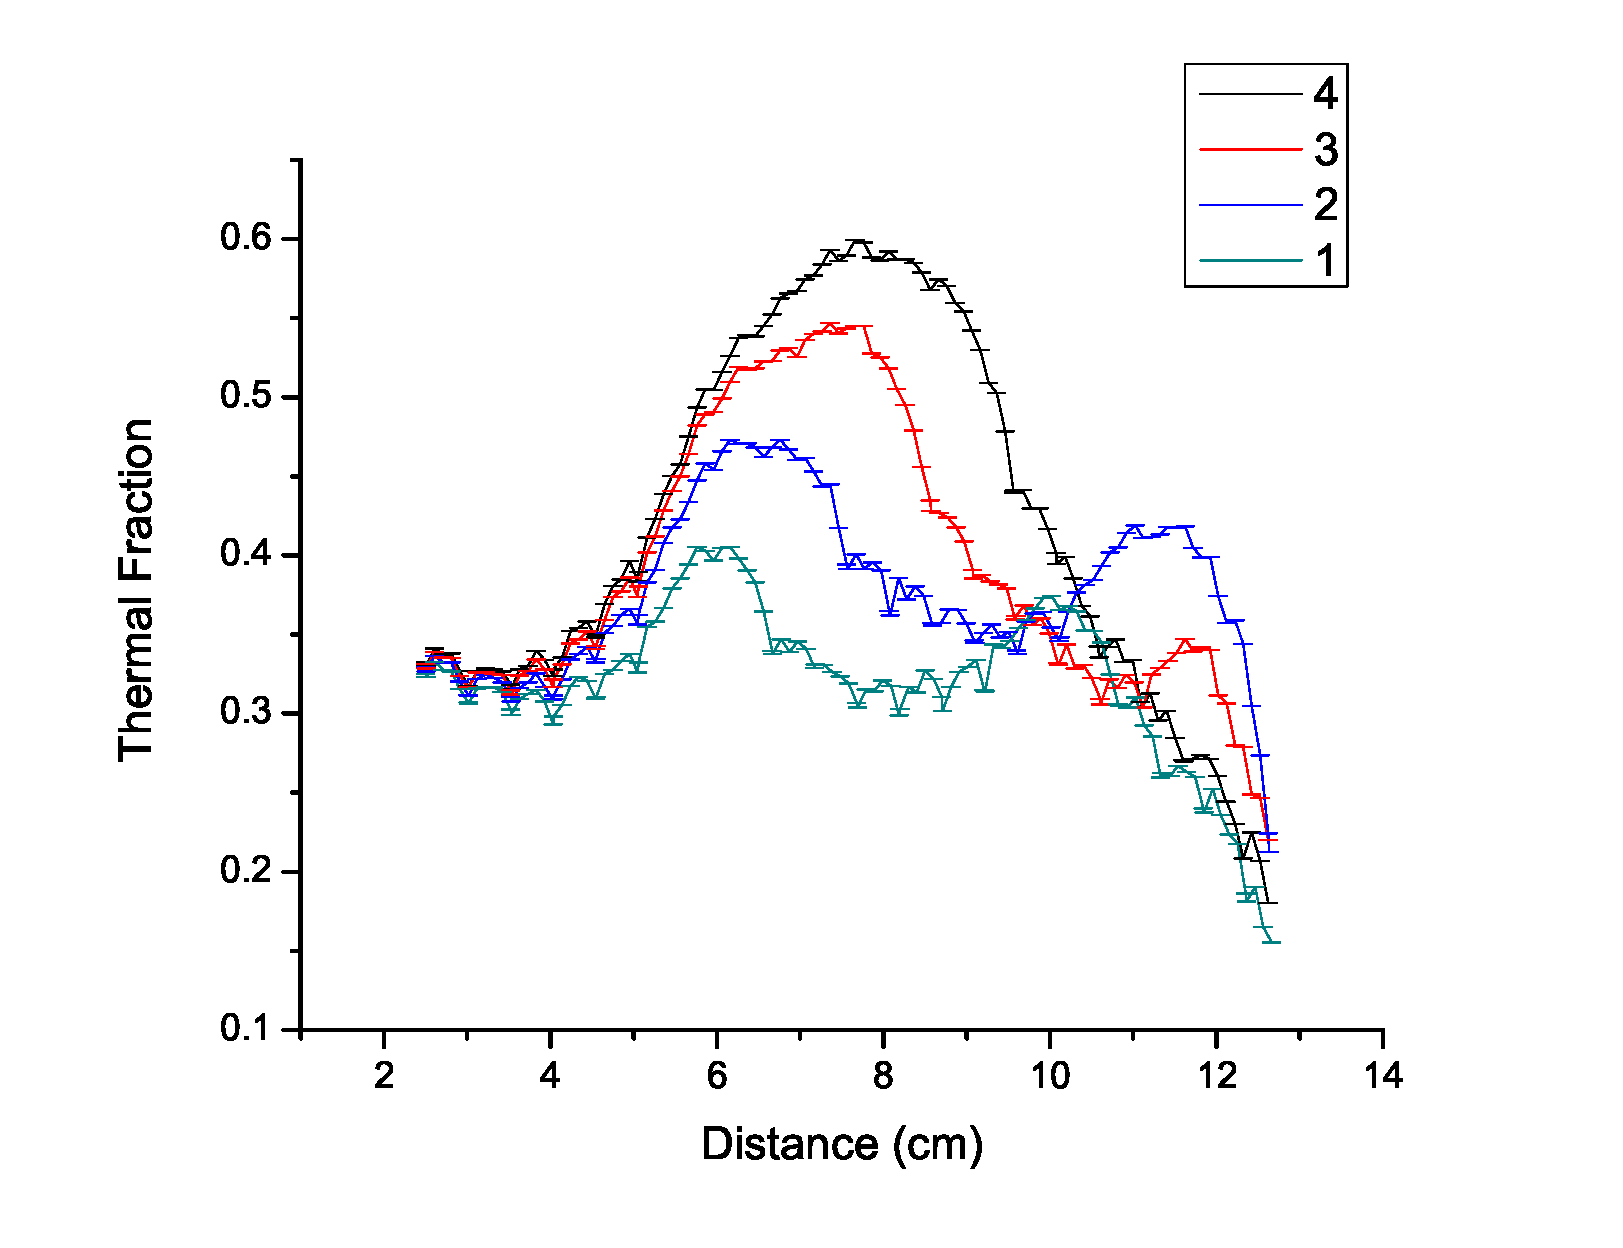
\includegraphics[width=\textwidth]{RPM8Opt_TF_6Assm.eps}
    \caption{6 Films per Assembly}
	\end{subfigure}

	\caption{Thermal Flux Profiles for Various Assemblies}
	\label{fig:ThermalFlux}
\end{figure}
\subsection{Optimized Detector Configuration}
The results of the genetic algorthim are shown below. 
Some of the search spaces were run multiple times, and what is shown is the majority vote of the algorthim on what the answer should be.
\begin{table}
  \begin{minipage}{\textwidth}
    \caption[Genomes of Optimized Geometries and Performace]{Optimized Geometries and Detector Performance\footnote{Subject to the given constraints}}
    \label{tab:GeneticOptimizedGeo}
    \centering
    \begin{tabular}{ c | c c c c}
        Genome &Assemblies&Films &Mass \iso[6]{Li} &Count Rate\\
        \hline
        \hline
        \verb+010+&1&4&16.75 &  0.175 \\
        \verb+0100+&1&4&16.75 & 0.197  \\
        \verb+01000+&1&3&12.56 & 0.230 \\
        \verb+01100+&2&6&25.13 & 0.157 \\
        \verb+0100000+&1&3&12.56& 0.229 \\
        \verb+01000000+&1&3&12.56&0.226 \\ 
        \hline
        \verb+0010000000+&1&3&& \\
        \hline
        13&2&&& \\
        26&1&&& \\
    \end{tabular}
    \end{minipage}
\end{table}
